\documentclass{beamer}

\mode<presentation> {
  \usetheme{Frankfurt}
  \setbeamercovered{transparent}
}

\usepackage[utf8]{inputenc}
\usepackage{graphicx}
\usepackage{subfig}
\usepackage[czech]{babel}

\title{Mobilní aplikace Florbalový trenér pro iOS}
\author{Jakub Olejník \\
\emph{vedoucí} Ing. Josef Gattermayer}
\institute[ČVUT FIT]{Katedra softwarového inženýrství\\
Fakulta informačních technologií\\
ČVUT v Praze}
\date{19.~6.~2014}

\begin{document}

\begin{frame}
  \titlepage
\end{frame}

\section{Zadání práce}

\begin{frame}
  \frametitle{Obsah}
  \tableofcontents[currentsection]
\end{frame}

\subsection{Motivace}
\begin{frame}
\frametitle{Motivace}

\begin{itemize}
  \item aplikace zaměřená na florbal neexistuje
  \item aplikace pro jiné sporty nepodporují florbalovou notaci
  \item odpadají nevýhody využití klasické kreslicí tabule
\end{itemize}

\end{frame}

\subsection{Zadání}
\begin{frame}
\frametitle{Zadání}

\begin{itemize}
  \item analýza podobných aplikací
  \item analýza požadavků vybraných trenérů
  \item UML modely
  \item wireframy
  \item specifikace
  \item prototyp aplikace
  \item akceptační test
\end{itemize}

\end{frame}

\section{Podobné aplikace}

\begin{frame}
  \frametitle{Obsah}
  \tableofcontents[currentsection]
\end{frame}

\subsection{CoachNote Hockey And Ringette}

\begin{frame}
\frametitle{CoachNote}

  \begin{figure}[H]
    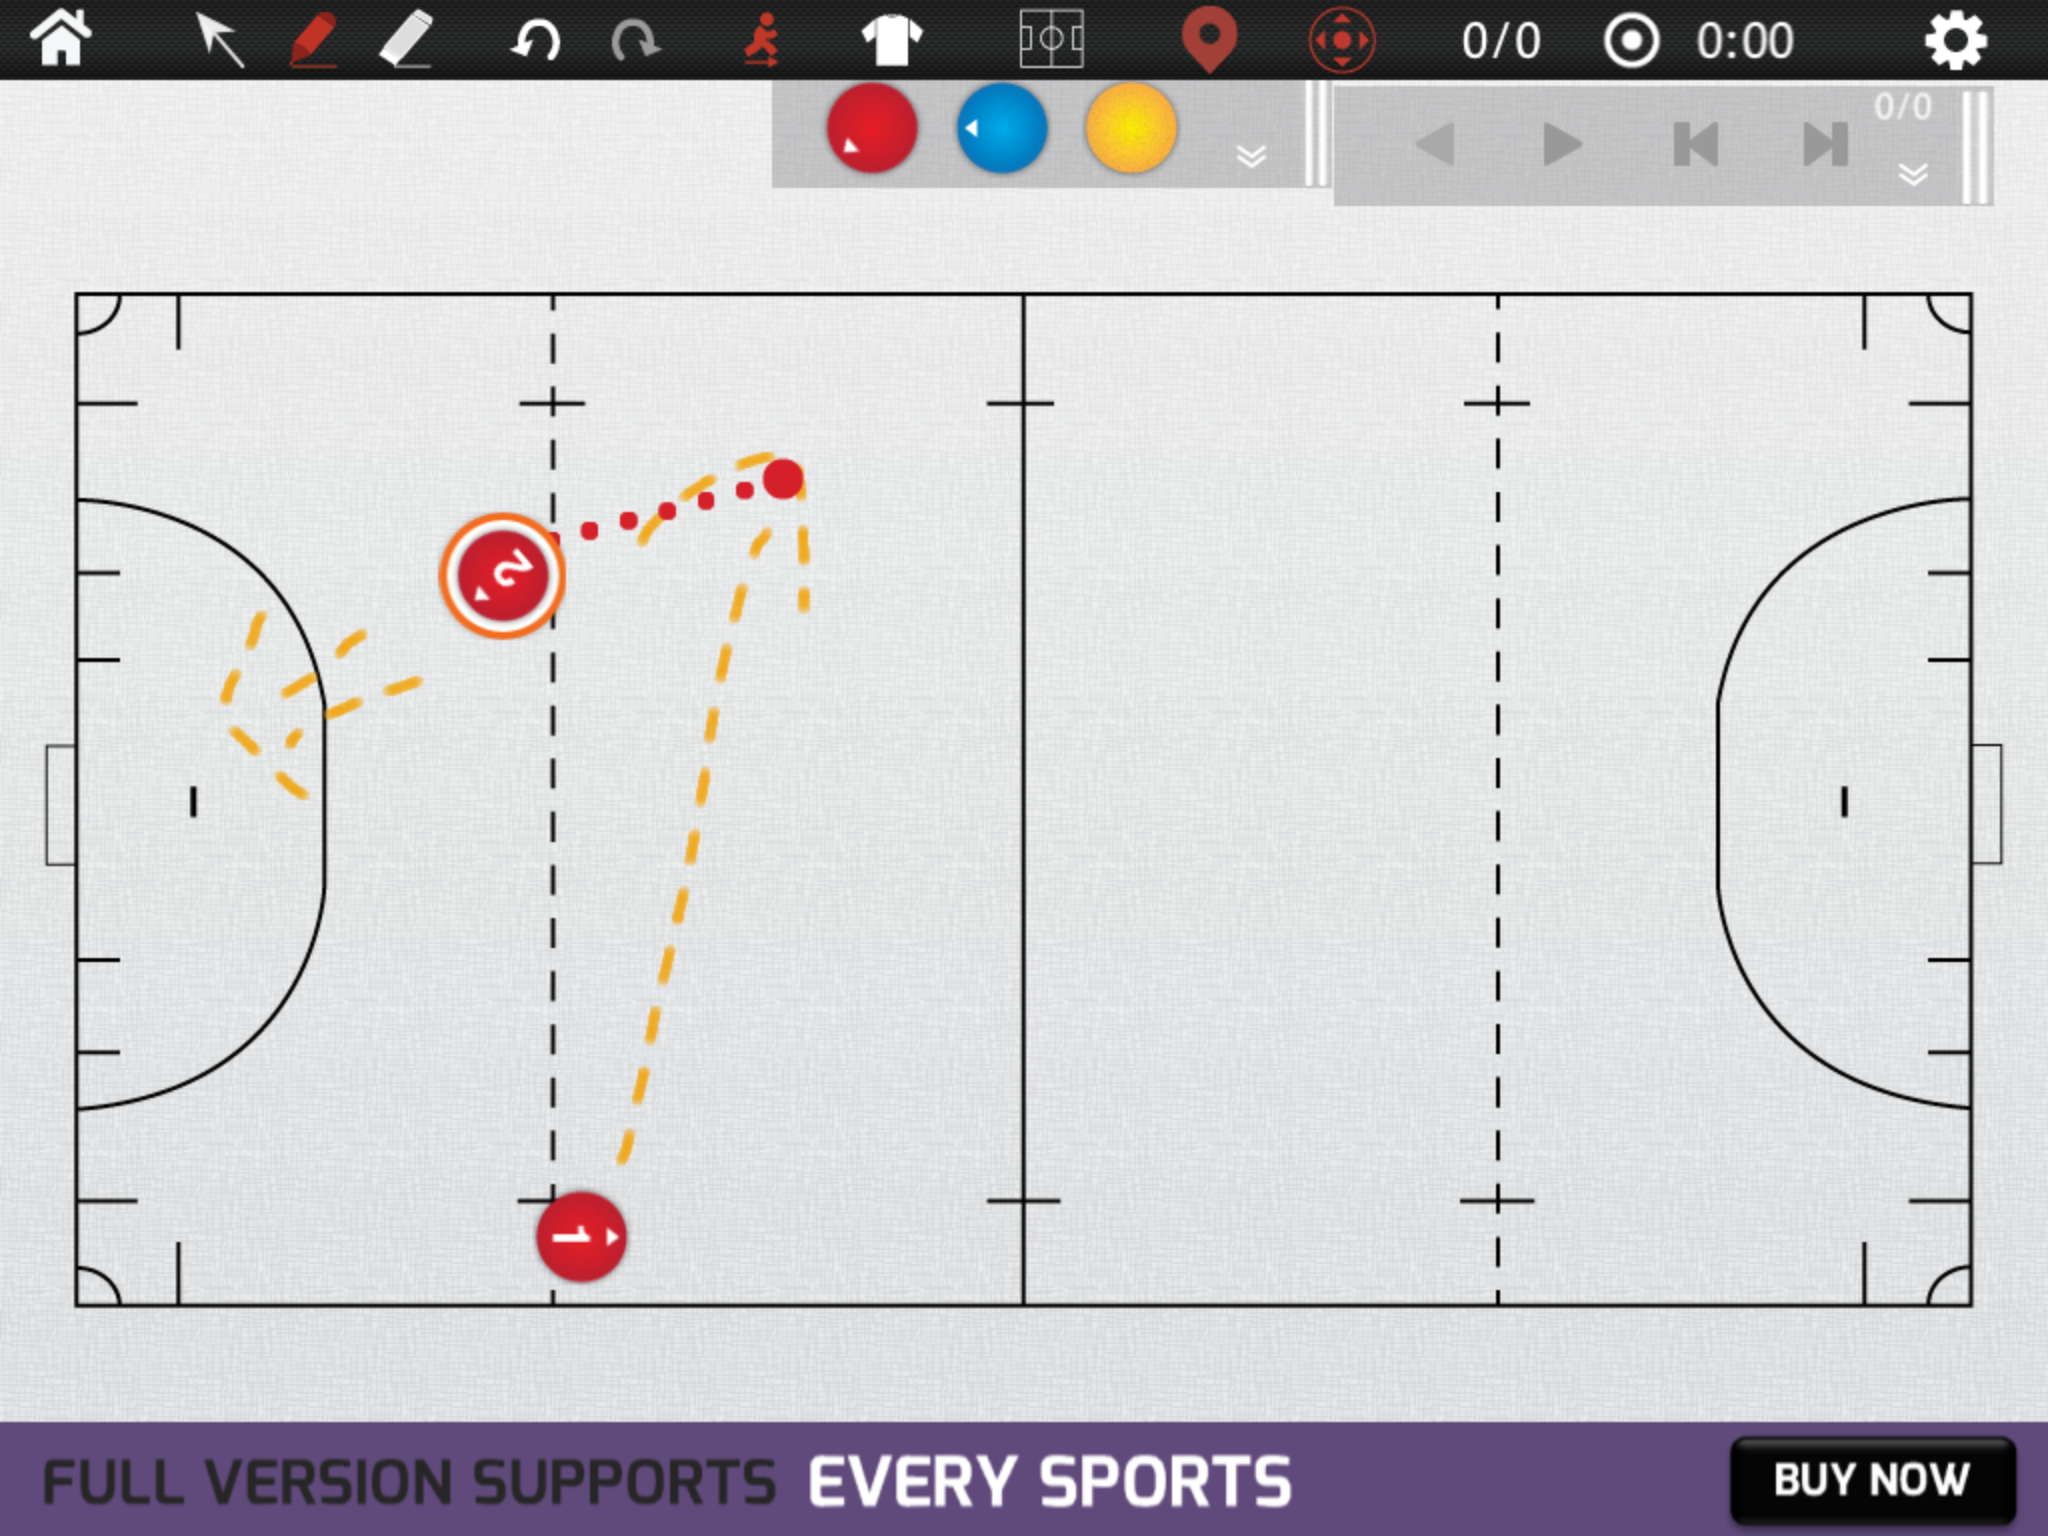
\includegraphics[width=.8\textwidth]{img/IMG_0011}
    \caption{Uživatelské rozhraní aplikace CoachNote}
    \label{pic:coachnote}
  \end{figure}

\end{frame}

\subsection{IceHockey Board Free}
\begin{frame}
\frametitle{IceHockey Board}

  \begin{figure}[H]
    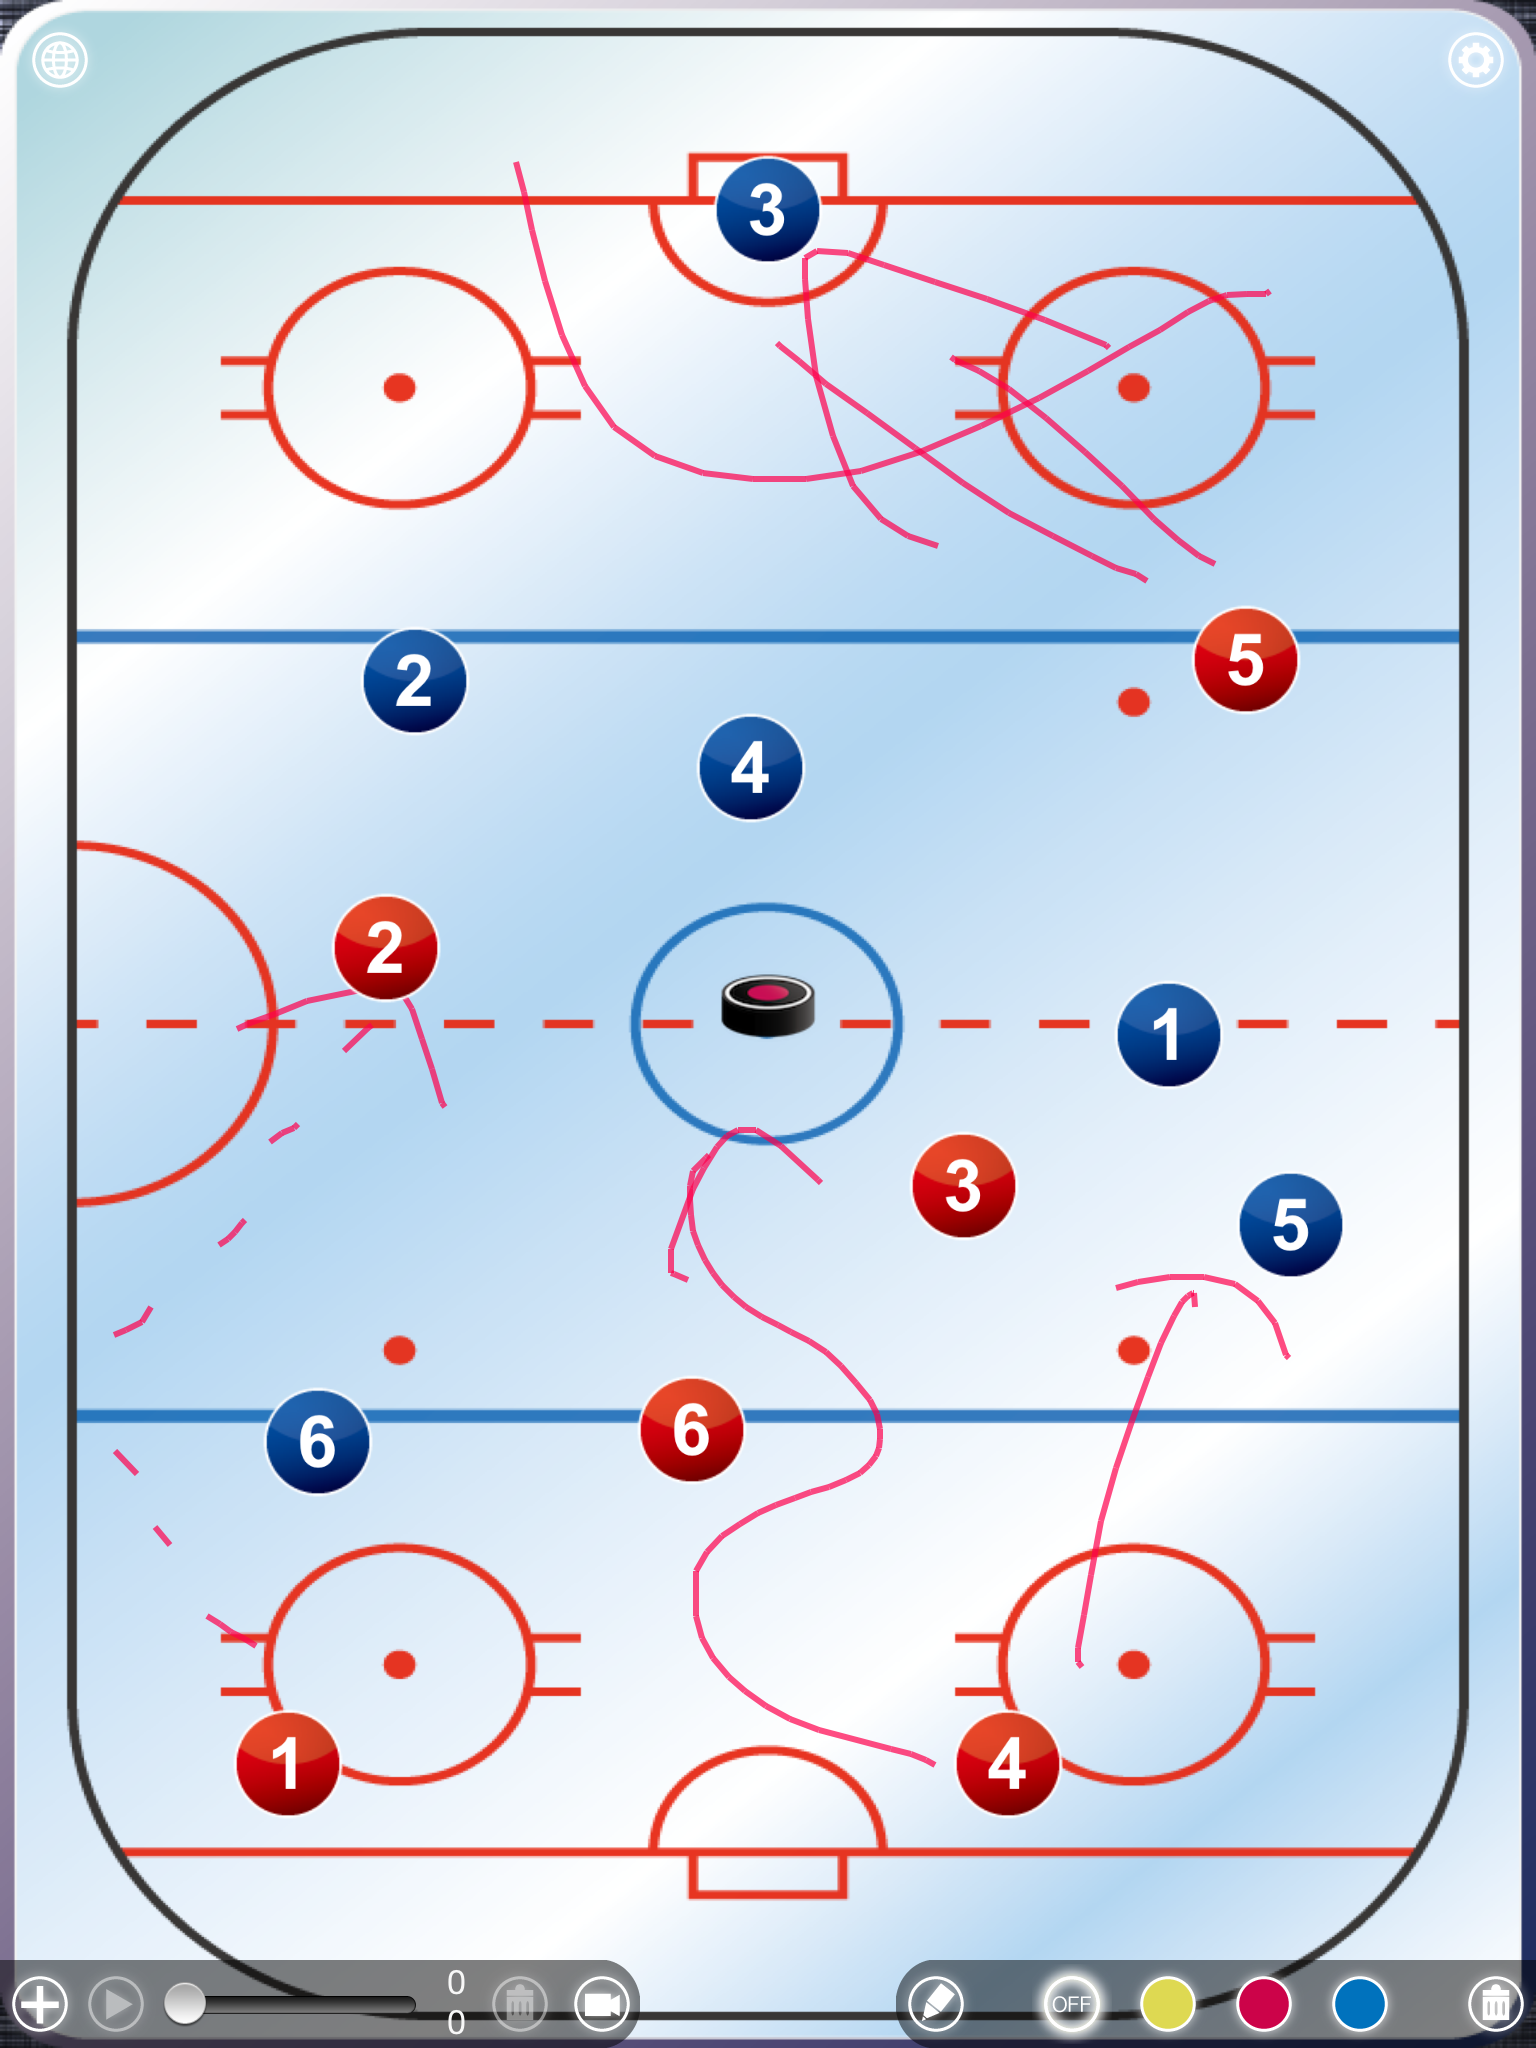
\includegraphics[height=.6\textheight]{img/IMG_0018}
    \caption{Uživatelské rozhraní aplikace IceHockey Board Free}
    \label{pic:icehockeyboardfree}
  \end{figure}

\end{frame}

\subsection{My Field Hockey Coach Free}
\begin{frame}
\frametitle{My Field Hockey Coach}
  \begin{figure}[H]
    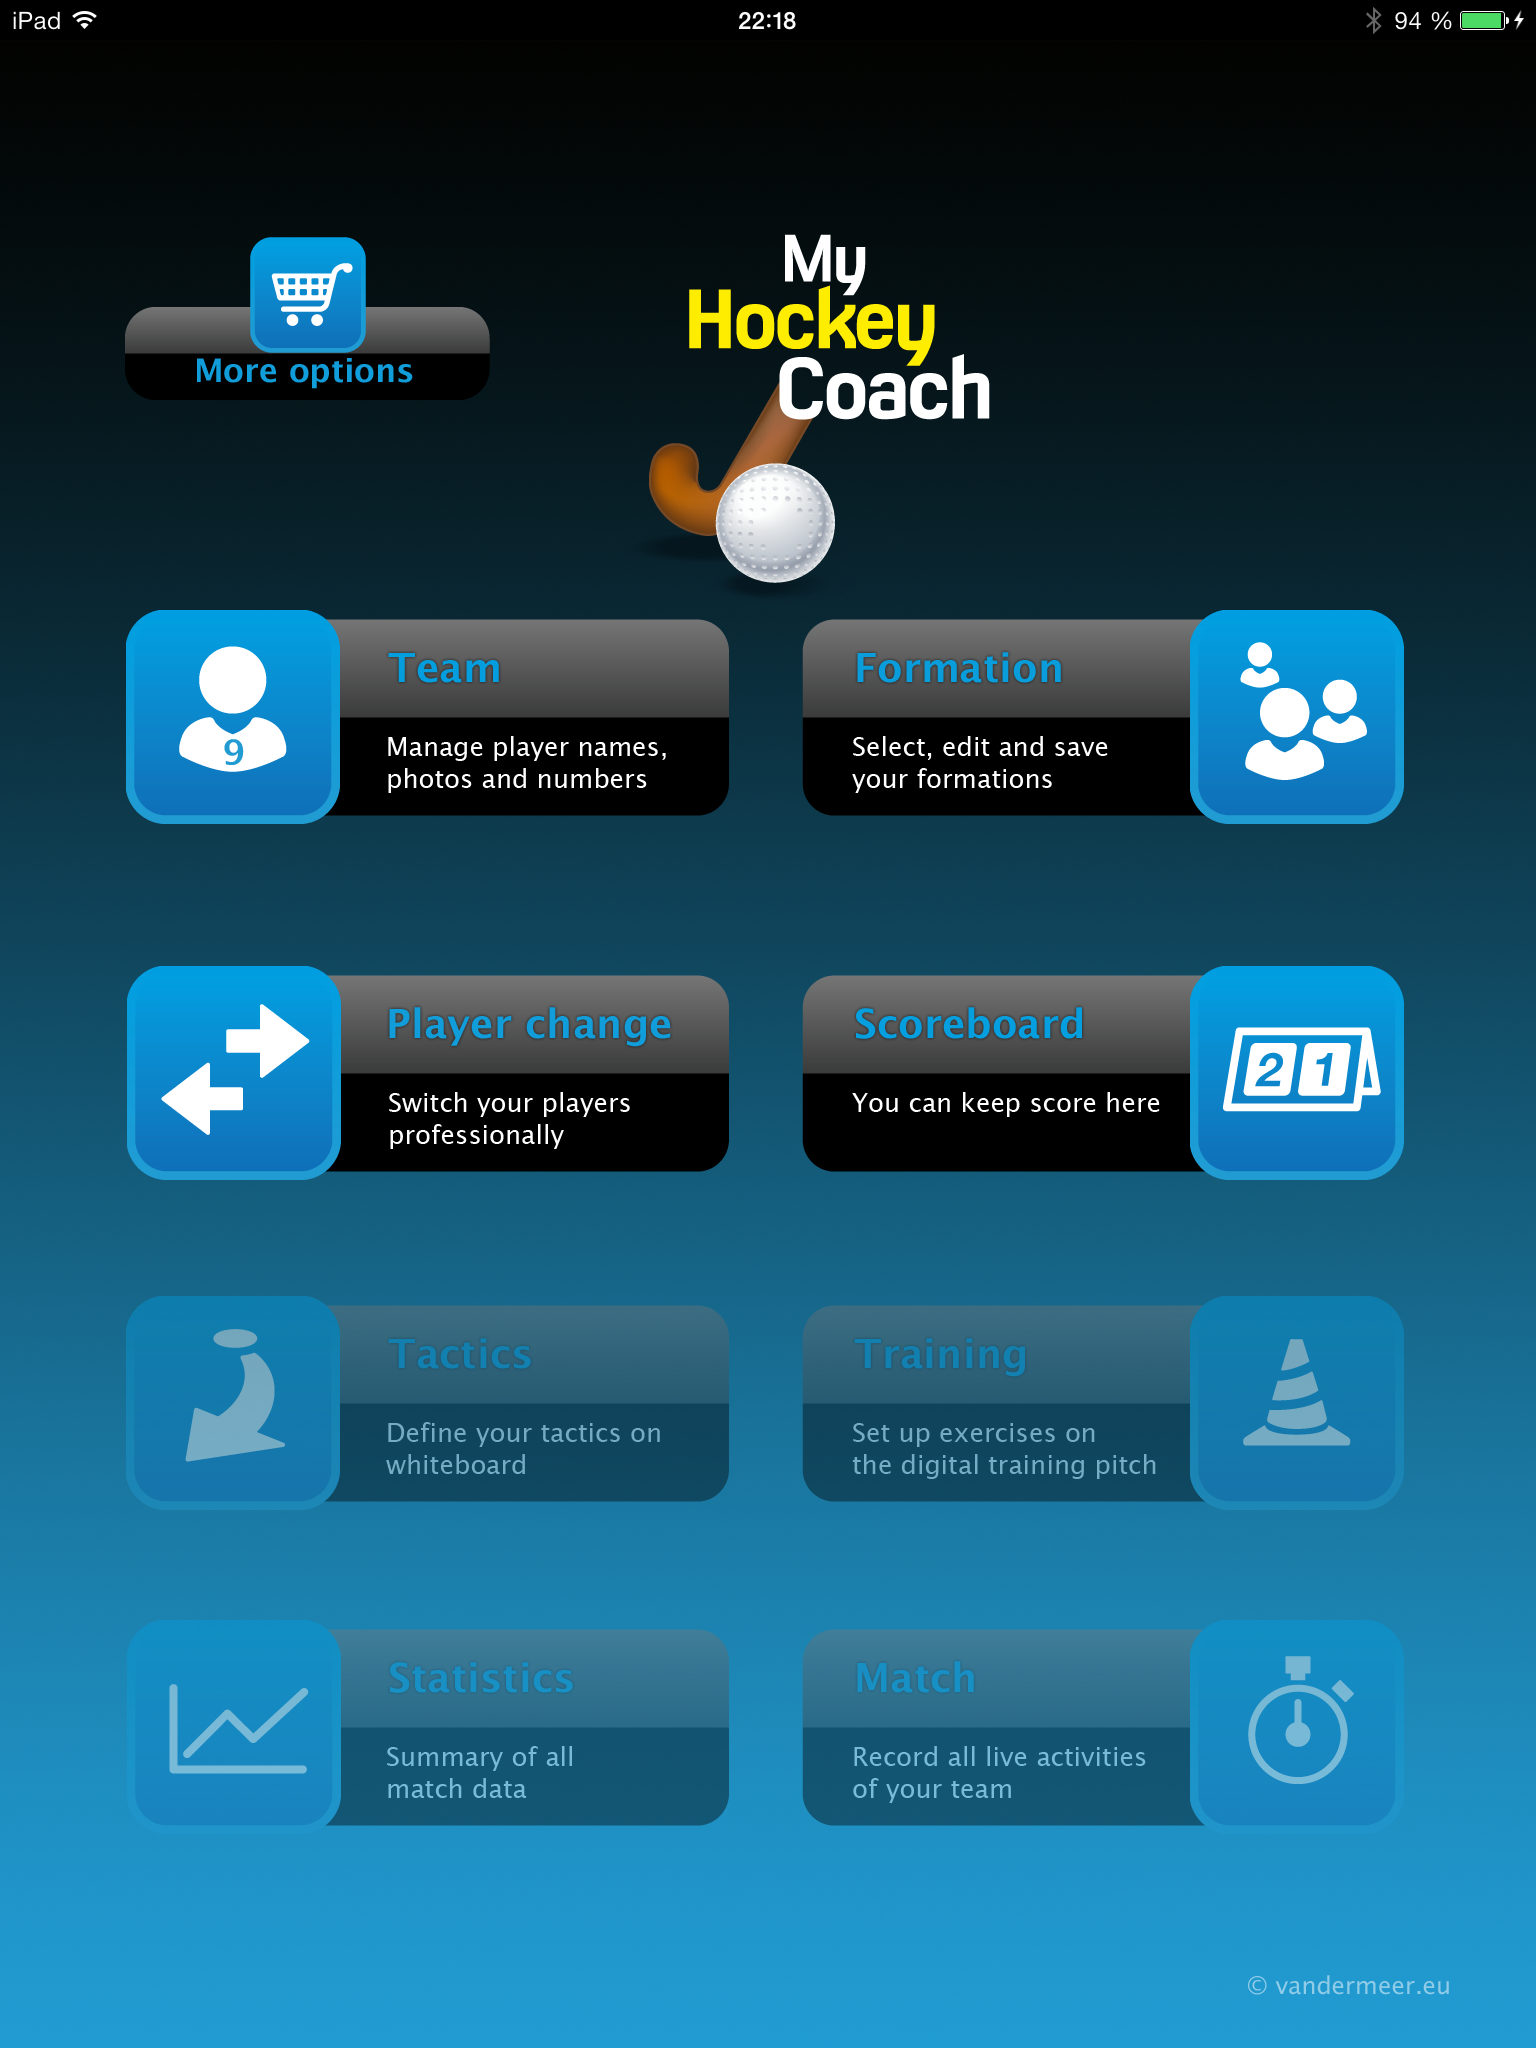
\includegraphics[height=.6\textheight]{img/IMG_0019}
    \caption{Uživatelské rozhraní aplikace My Field Hockey Coach Free}
    \label{pic:myfieldhockeycoachfree}
  \end{figure}
\end{frame}

\subsection{Exercise drawer}
\begin{frame}
\frametitle{Exercise drawer}
  \begin{figure}[H]
    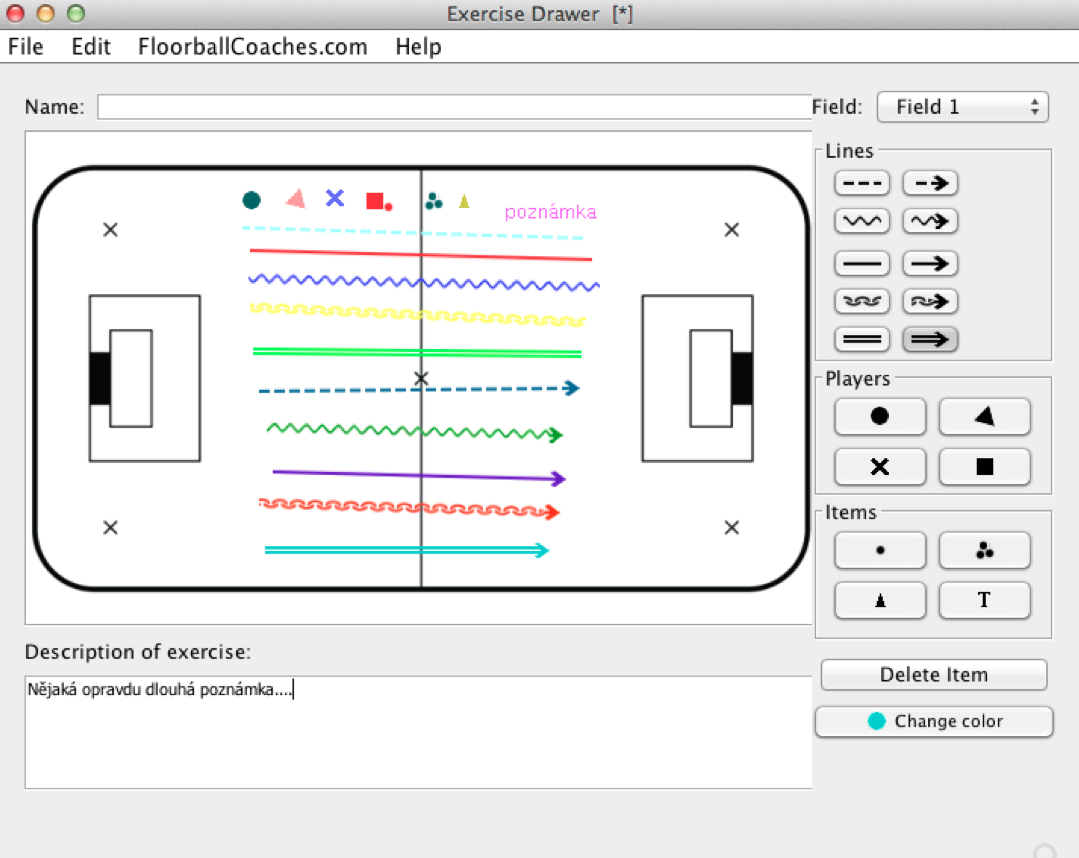
\includegraphics[height=.6\textheight]{img/exercise_drawer}
    \caption{Uživatelské rozhraní aplikace Exercise drawer}
    \label{pic:exercisedrawer}
  \end{figure}
\end{frame}

\section{Prototyp}

\subsection{Uživatelské rozhraní}

\begin{frame}
  \frametitle{Uživatelské rozhraní}

  \begin{figure}[H]

    \centering
    \subfloat[Hlavní nabídka]{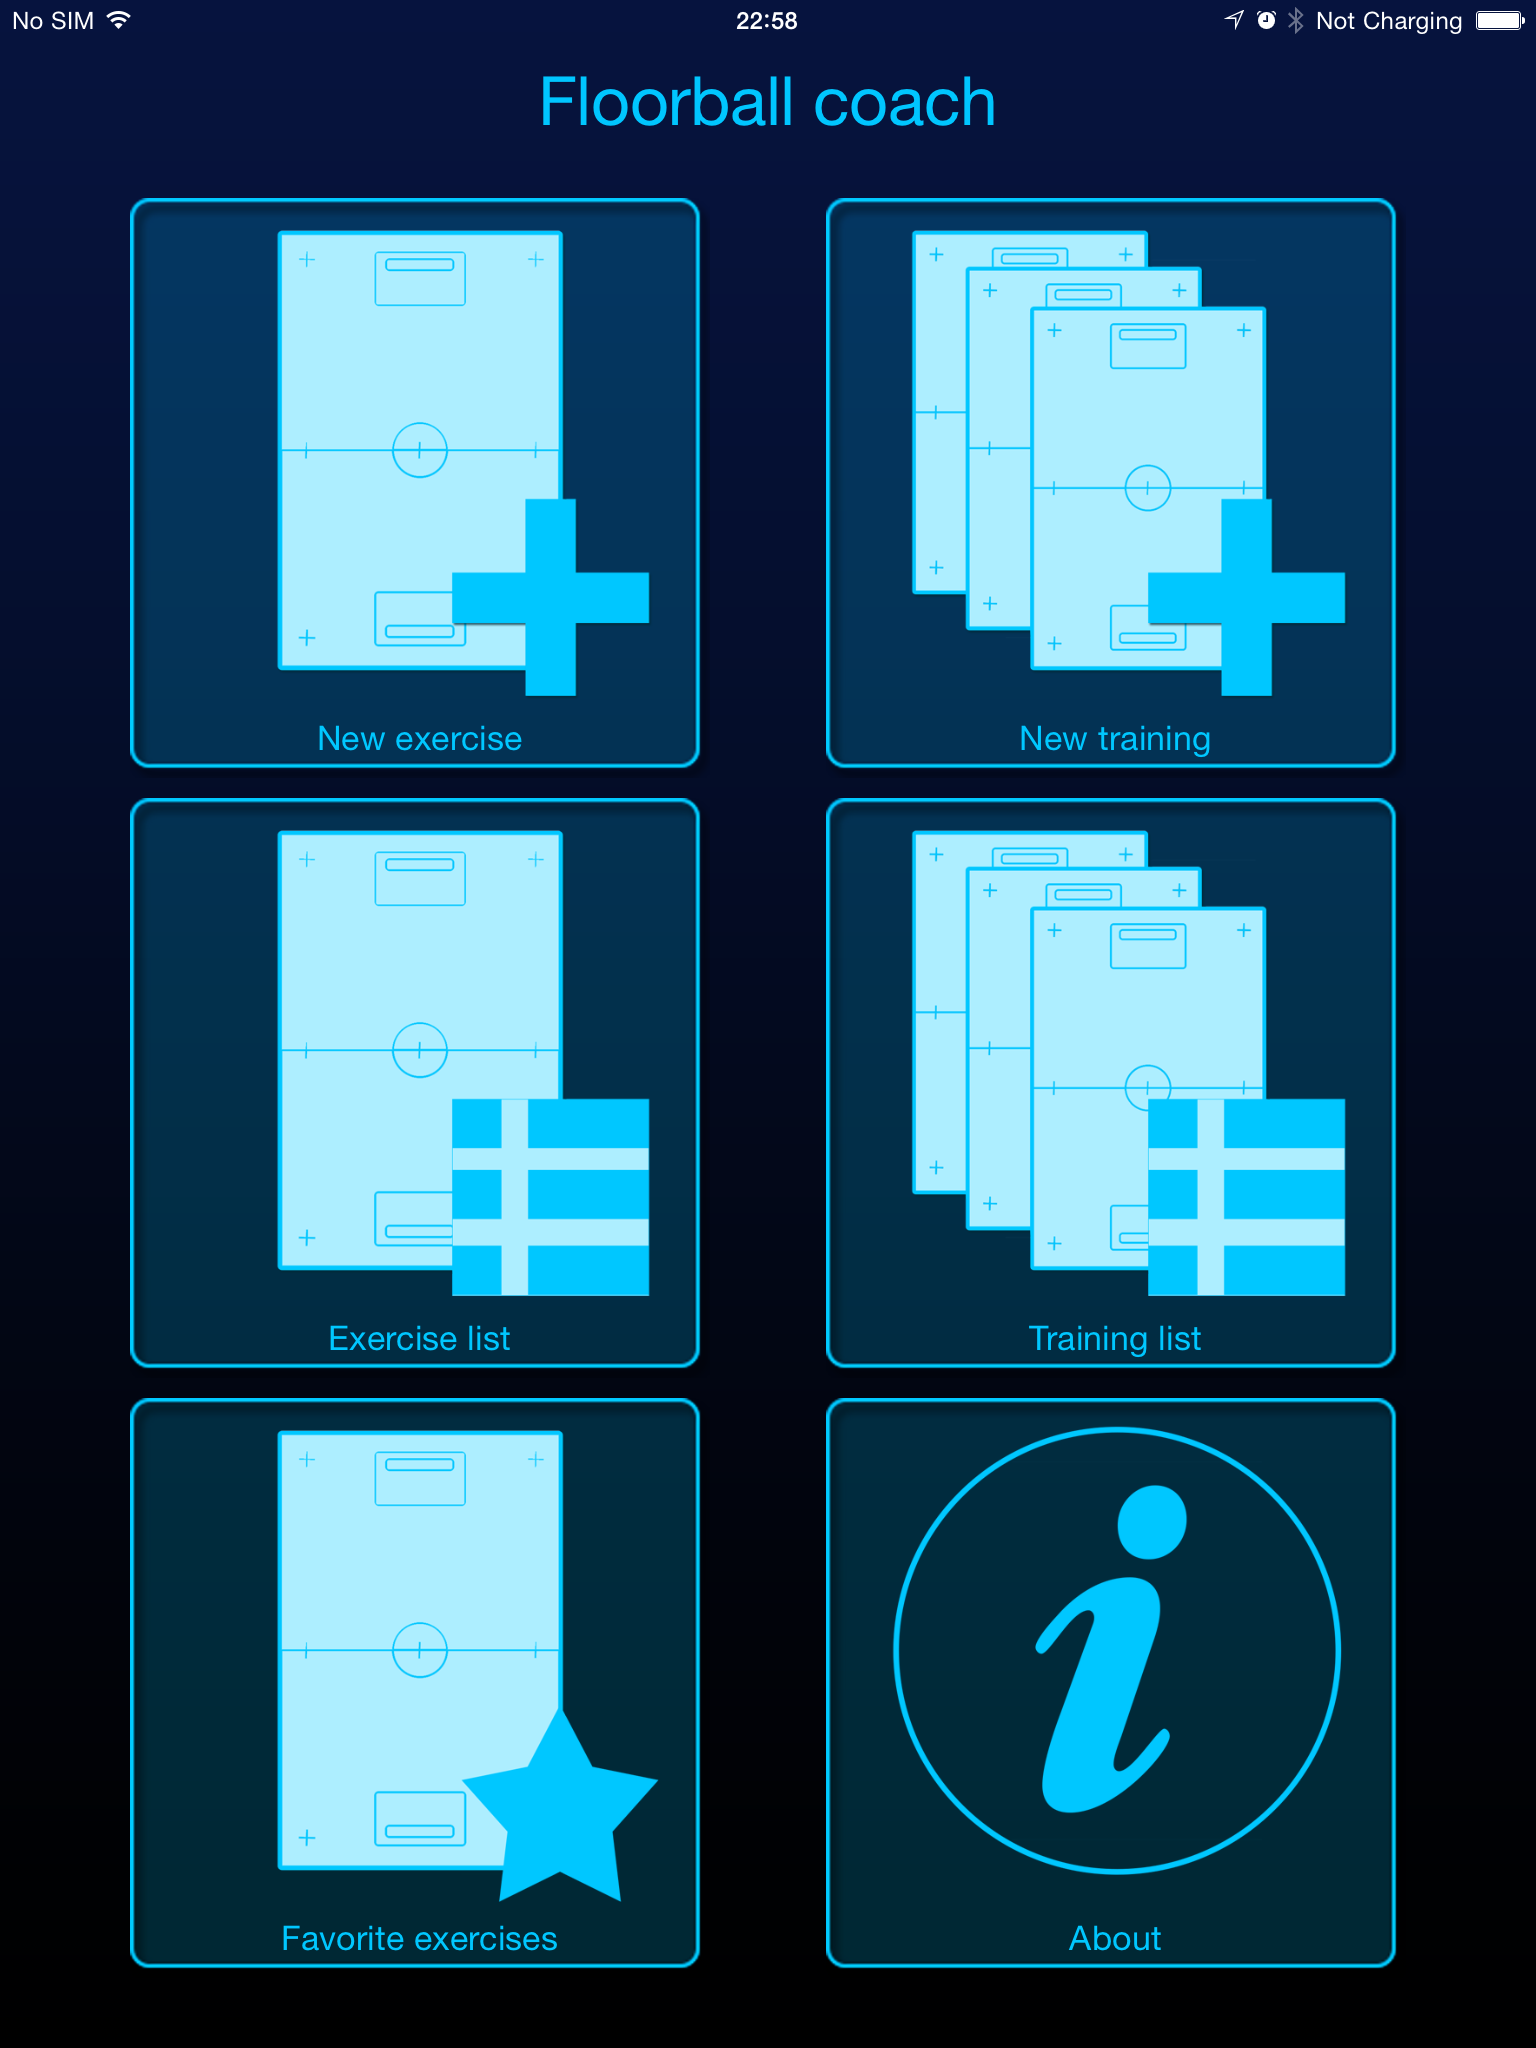
\includegraphics[width=0.4\textwidth]{img/IMG_0277}}
    \hfil
    \subfloat[Obrazovka kreslení]{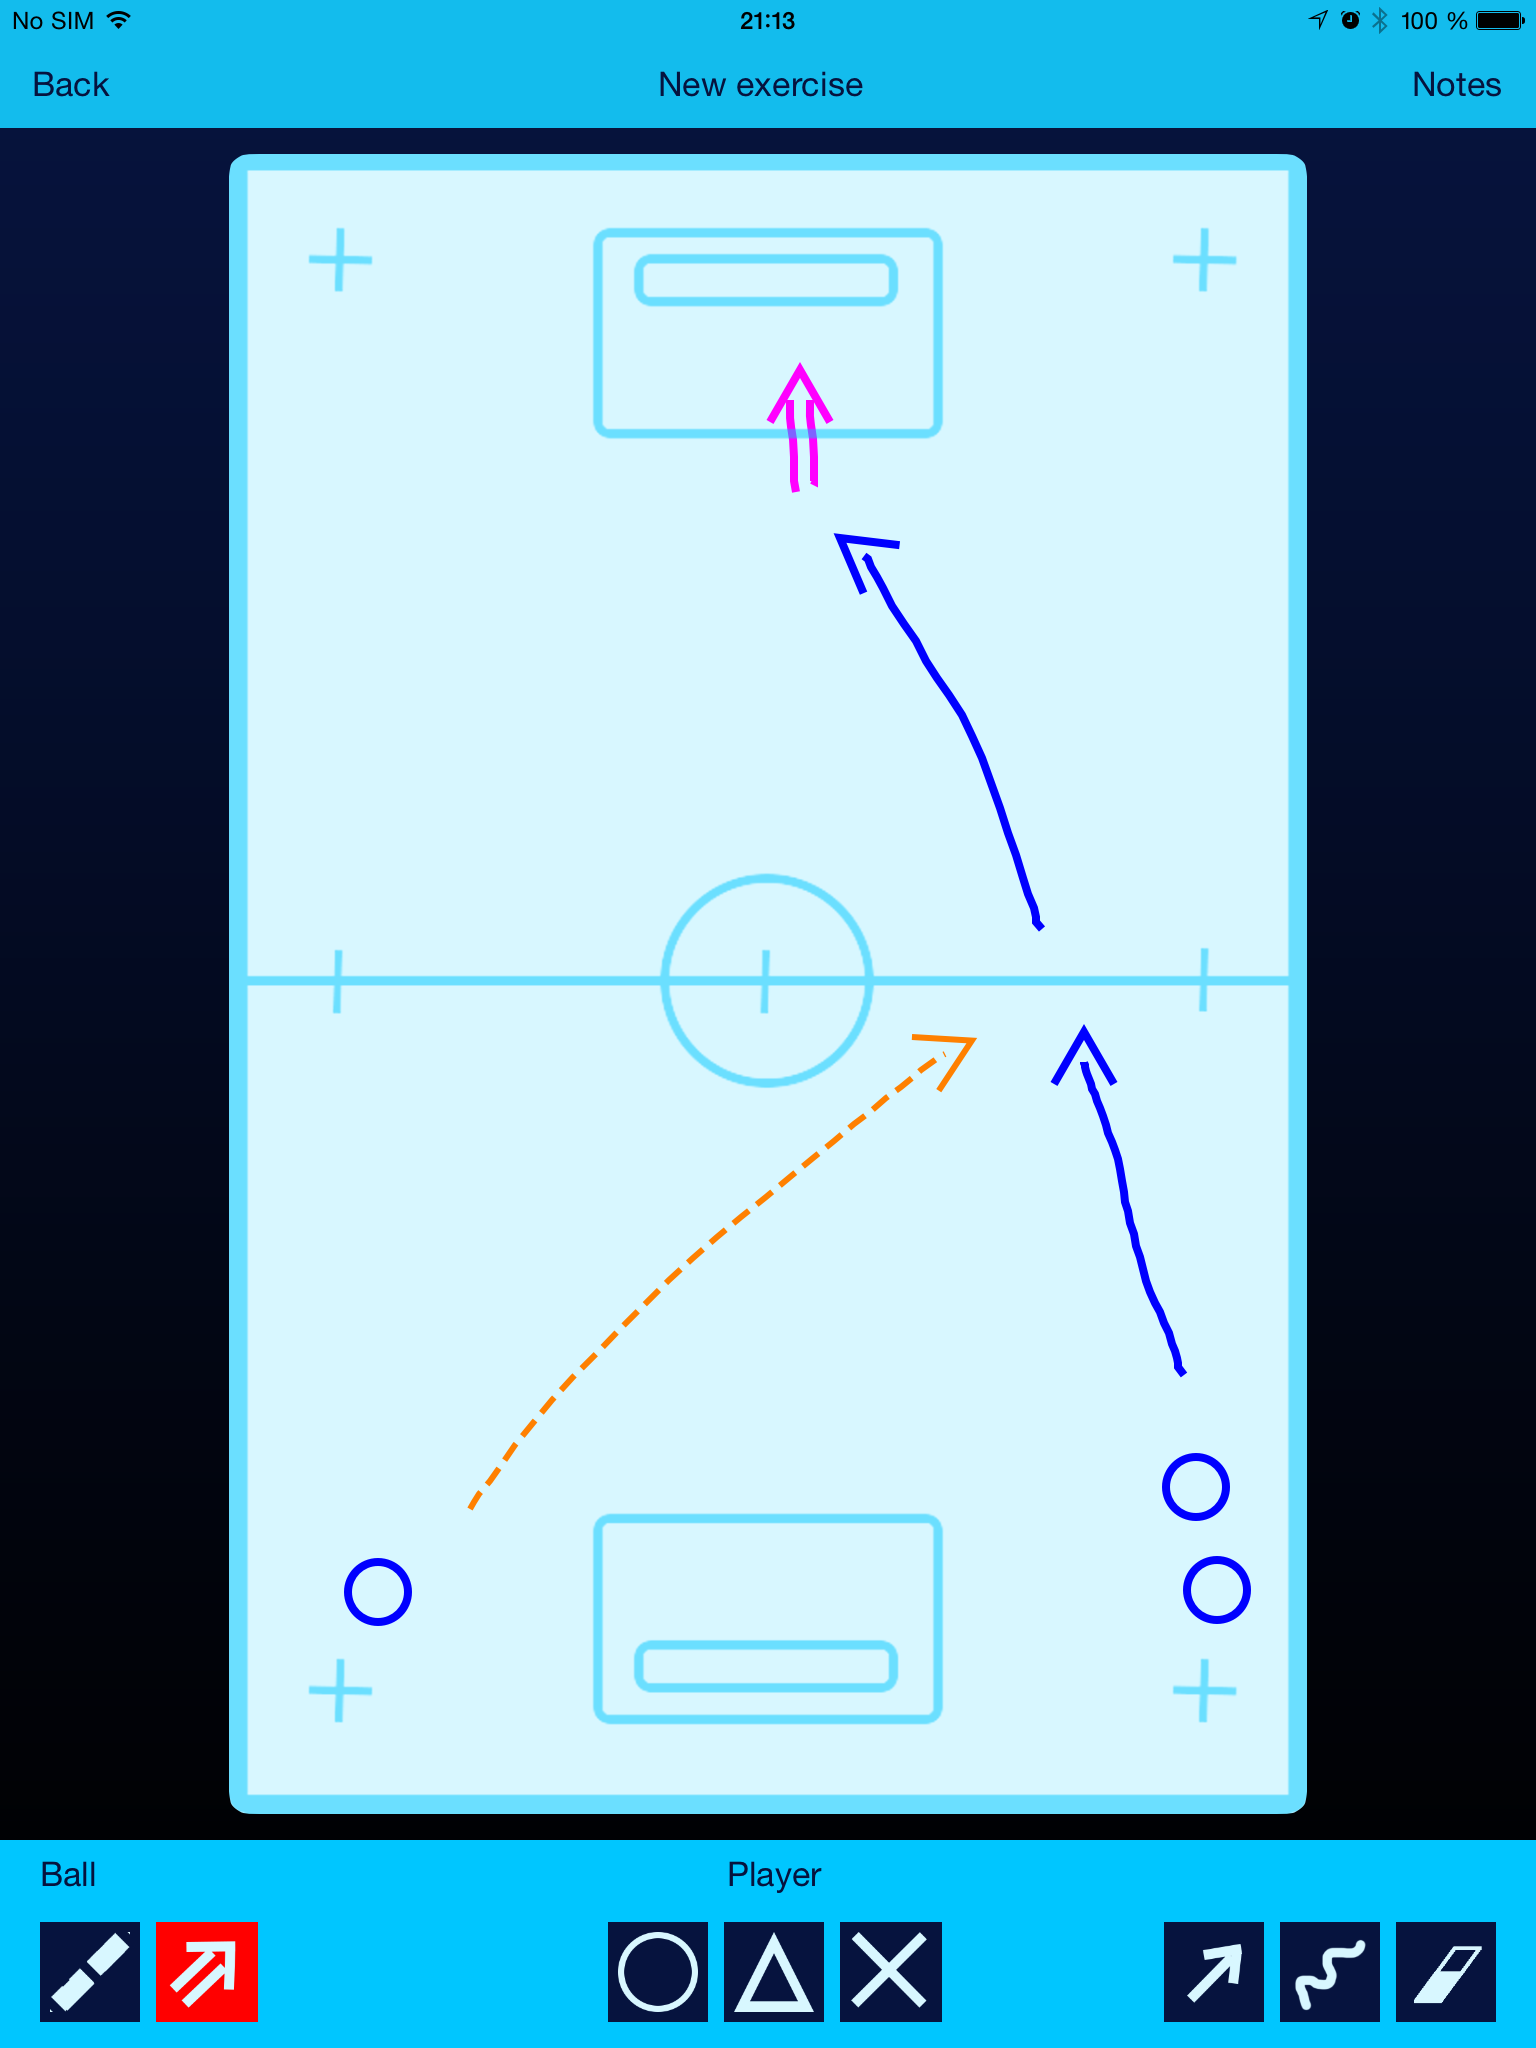
\includegraphics[width=0.4\textwidth]{img/IMG_0276}}

    \caption{Uživatelské rozhraní navržené aplikace}
    \label{pic:prototype_ui}
  \end{figure}
\end{frame}

\subsection{Funkcionalita}

\begin{frame}
  \frametitle{Funkcionalita}

  \begin{itemize}
    \item volné kreslení na hřiště
    \item předpřipravené nástroje
    \item textové poznámky
    \item perzistentní ukládání cvičení
    \item seskupování cvičení do tréninků
  \end{itemize}
\end{frame}

\section{Testování}

\begin{frame}
  \frametitle{Testování}
  \begin{itemize}
    \item unit testy
    \item testy uživatelského rozhraní
    \item akceptační testy
  \end{itemize}
\end{frame}

\section{Závěr}

\begin{frame}
  \frametitle{Obsah}
  \tableofcontents[currentsection]
\end{frame}

\subsection{Shrnutí}

\begin{frame}
  \frametitle{Shrnutí}

  \begin{block}{Úkol}
    \begin{itemize}
      \item návrh aplikace pro zlepšení vedení florbalových tréninků
      \item analýza existujících řešení
      \item analýza požadavků budoucích uživatelů
      \item akceptační test
    \end{itemize}

  \end{block}

  \begin{block}{Zhodnocení}
    \begin{itemize}
      \item aplikace dokončena a připravena pro submit na App Store
      \item analýza soustředěna především na podobné aplikace a požadavky budoucích uživatelů
      \item akceptační test doplněn také o testy uživatelského rozhraní a unit testy
    \end{itemize}
  \end{block}
\end{frame}

\subsection{Obhajoba}

\begin{frame}
  \frametitle{Jakým způsobem a s jakými konkrétními výsledky byly provedeny akceptační testy?}

  Způsoby:

  \begin{enumerate}
    \item vývojář podle připraveného scénáře
    \item automatizace podle připraveného scénáře
    \item budoucí uživatel bez připraveného scénáře
  \end{enumerate}

  Výsledky:

  \begin{itemize}
    \item u prvních dvou způsobů bylo výstupem zda test dosáhl očekávaného výsledku
    \item třetí způsob byl kombinací akceptačního testu s testem uživatelského rozhraní a výstupem byl i komentář uživatele jak obtížné bylo se k očekávanému cíli dostat
  \end{itemize}

\end{frame}
\begin{frame}
  \frametitle{Bylo řešení konzultováno s budoucími uživateli i v průběhu analýzy, návrhu a/nebo implementace?}

  \begin{itemize}
    \item doplnění funkcí, popř. tipů na fuknce do aplikace během analýzy
    \item úpravy wireframů během návrhu
    \item zpětná vazba vybraných trenérů během implementace
  \end{itemize}
\end{frame}

\end{document}
